\subsection{Notation}
\TODO{Notation needs to be introduced in the background section}
We represent a decision tree by $T = (V, E, r)$ where $V$ is the set of nodes, $E$ the set of edges and
$r \in V$ is the root. For each node $n \in V$, we define the following.
\begin{enumerate}
    \item $threshold(n) \in \mathbb{R}$, the threshold value for $n$.
    \item $featureIndex(n) \in \mathbb{N}$, the feature index for $n$.
    \item $left(n) \in V$, the left child of $n$ or $\emptyset$ if $n$ is a leaf. If $left(n) \neq \emptyset$, then $(n, left(n)) \in E$.
    \item $right(n) \in V$, the right child of $n$ or $\emptyset$ if $n$ is a leaf. If $right(n) \neq \emptyset$, then $(n, right(n)) \in E$.
\end{enumerate}
We use $L \subseteq V$ to denote the set of leaves. % subseteq because tree could have single node

\subsection{Tiling}
\label{sec:Tiling}
% Treebeard vectorizes tree walks by grouping nodes of a decision tree into \textbf{\emph{tiles}}. The nodes in a tile are evaluated concurrently using vector instructions. Once the nodes of the current tile are evaluated, a look up table is used to compute which child of the current tile to move to next.
Treebeard groups nodes of the decision tree into \textbf{\emph{tiles}}. Tiling provides two benefits. 
\begin{enumerate}
  \item It allows the compiler to generate vector code to traverse trees. Section \ref{sec:Vectorization} describes how Treebeard does this.
  \item It enables spatial locality improvements by grouping together nodes that are likely to be accessed together. 
\end{enumerate}
Once nodes are grouped into tiles, an $n$-ary tree whose nodes are tiles is constructed. Treebeard then generates 
optimized code to walk this tree. The listing below shows at a high level how a tiled tree is walked (This is not 
true IR, but presented for clarity). 
\begin{lstlisting}[style=c++]
  ResultType Prediction_Function(...) {
    // ...
    Tile t = getRootTile(tree)
    while (!isLeaf(tree, t)) do {
      // Evaluate conditions of all nodes in the tile
      predicates = evaluateTilePredicates(t, rows[i])
      
      // Move to the correct child of the current tile
      t = getChildTile(tree, t, predicates) 
    }
    treePrediction = getLeafValue(t)
    // ...
  }  
\end{lstlisting}

To compute the prediction of the tree, the predicates of all nodes in the tile are computed simultaneously (line 6). 
Then, the computed predicate values are used to determine which child of the current tile to move to (in the 
$n$-ary tree). This section presents the details of tiling and how Treebeard's general tiling infrastructure 
can be used to develop tiling algorithms with different objectives (sections \ref{sec:UnifTiling}) and \ref{sec:ProbTiling}).
The details of how Treebeard lowers predicate evaluation and moving to the correct child to use vector instructions 
are described in section \ref{sec:Vectorization}.

\subsection{Tiles and Tree Tiling}
\label{sec:ValidTiling}
A \textbf{\emph{tile}} is a collection of connected non-leaf nodes of a decision tree. The path connecting any pair of nodes
in the tile must be contained fully within the tile. The \textbf{\emph{tile size}} $n_t$ is the number of nodes contained in a tile.

A \textbf{\emph{tiling}} $\mathcal{T}$ of the tree $T = (V, E, r)$ with tile size $n_t$ is a partition $\{ T_1, T_2, ... ,T_m \}$ of the set $V$ such that 
\begin{enumerate}
    \item $T_1 \cup T_2 ... \cup T_m = V$
    \item $T_i \cap T_j = \emptyset$ for all $i, j \in [1, m]$ and $i \neq j$
    \item Tiles are \textbf{connected}, i.e. for an $u, v \in T_i$, there is a (undirected) path connecting $u$ and $v$ fully contained in $T_i$.
\end{enumerate} 

We say a tiling $\mathcal{T}$ is a \textbf{\emph{valid tiling}} iff
\begin{enumerate}
  \item $|T_i| \leq n_t$ for all $i \in [1, m]$
  \item $\forall l \in L$ : $l \in T_i \rightarrow v \notin T_i \;\; \forall v \in V \backslash \{l\}$
  \item Tiles are \textbf{maximal}, i.e. if $|T_i| < n_t$, then there is no $v \in V\backslash \{ T_i \cup L \}$ such that $(u, v) \in E$ for some $u \in T_i$. 
\end{enumerate}

\subsection{Tiled Trees}
A tiling transformation communicates the tiling to the Treebeard infrastructure by assigning a tile ID to each node in the decision tree. Using these tile IDs, Treebeard checks the validity of the tiling and then contructs a tree whose nodes are tiles. We call this tree the \textbf{\emph{tree of tiles}}. \TODO{We need a better name for this}
Figure \ref{Fig:ValidTilingTileSize3} shows a valid tiling with tile size 3 and the tree of tiles constructed by Treebeard. Three nodes are grouped into each of the tiles $t_1$ and $t_2$ as shown. Each tile is collapsed into a single node in the tree of tiles. However, each leaf in the original tree becomes a leaf in the tree of tiles.

\begin{figure}
  \centering
  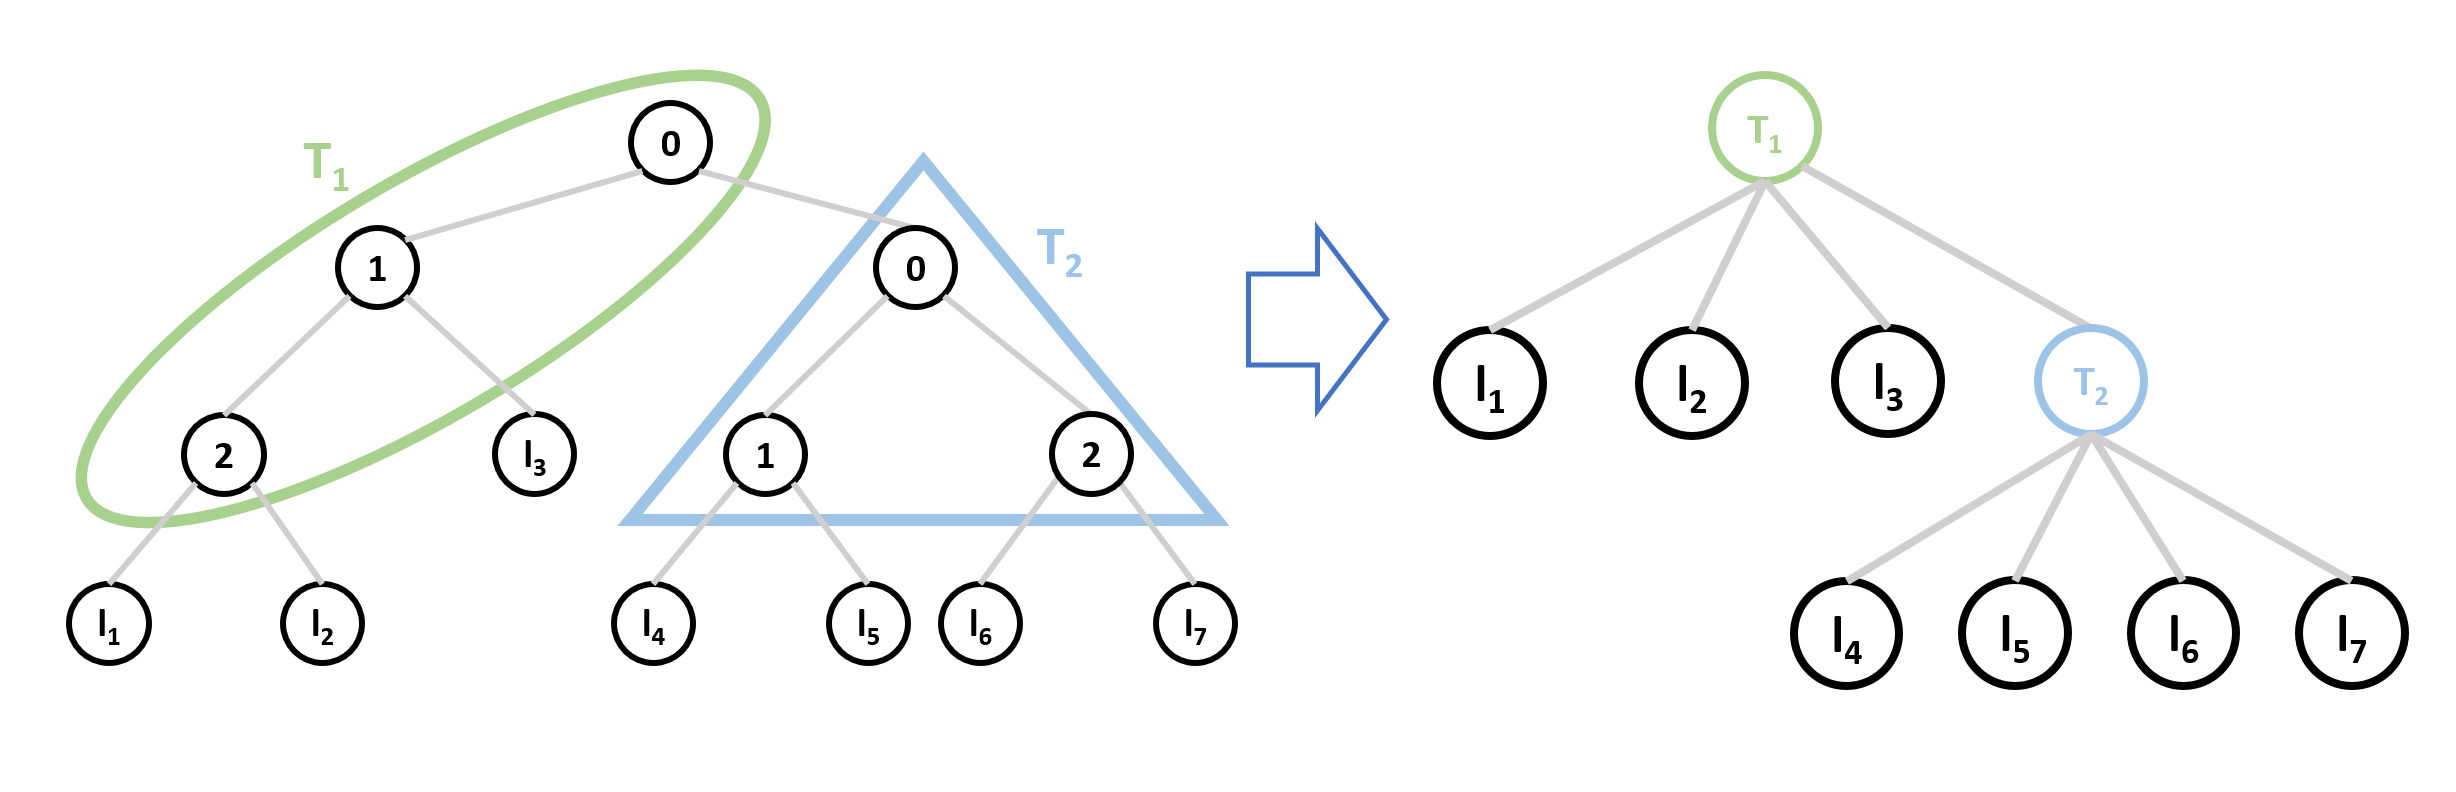
\includegraphics[width=\linewidth]{figures/TiledTree_Size3.PNG}
  \caption{Example of a valid tree tiling with tile size $n_t=3$}
  \label{Fig:ValidTilingTileSize3}
\end{figure}

Treebeard maintains the following invariants.
\begin{enumerate}
  \item All tiles in a tree are the same size $n_t$. If the tiling produces any smaller tiles, these are padded by inserting dummy nodes to make them the required size.
  \item Nodes within tiles are always ordered in level order and left to right within a level. The numbering of the nodes in the above diagram shows this node order.
  \item Children of a node are numbered from left to right (regardless of level). For example, $l_1$ is the first child of $t_1$, $l_2$ is the second and so on.
\end{enumerate}
    
